\section{CTF3 objectives}

\begin{figure}[!h]
\begin{center}
%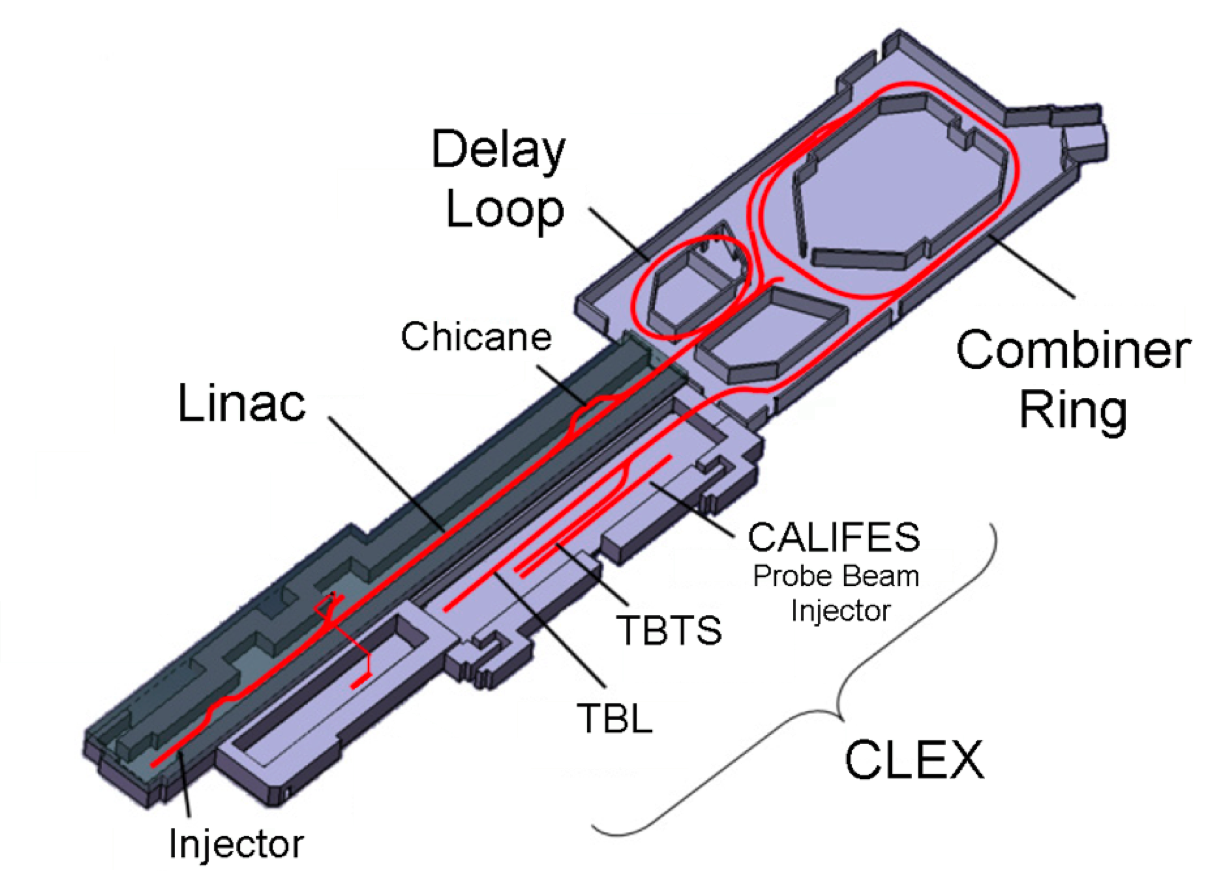
\includegraphics[height=8.4cm,natwidth=610,natheight=642]{CTF3_layout.png}
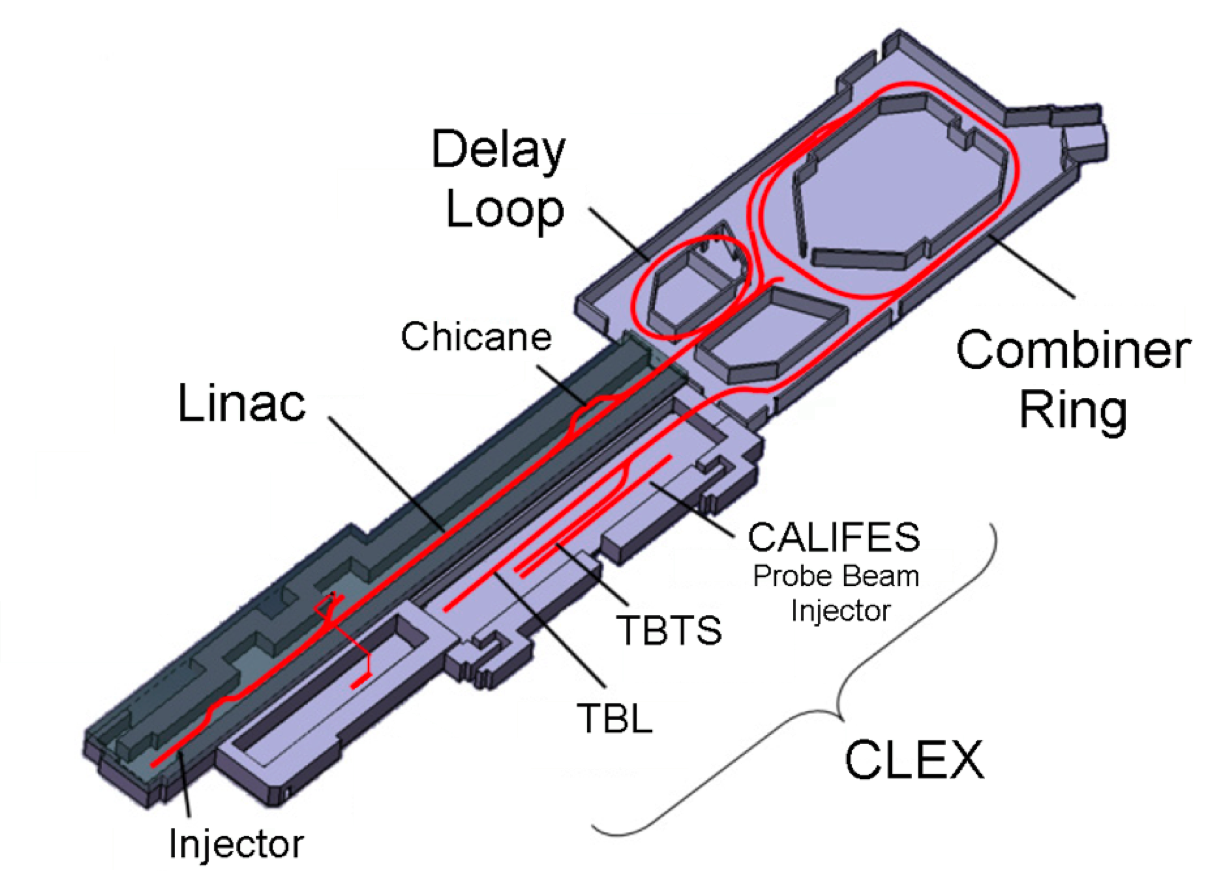
\includegraphics[height=8.4cm]{CTF3_layout.png}
\end{center}
\caption{Layout of the CTF3 complex.}
\label{fig:ctf3layout}
\end{figure}

CTF3 (CLIC Test Facility 3) was a test facility aiming to experimentally demonstrate the feasibility 
of the CLIC technology~\cite{bib:CDR}.
The main points were the generation of the high current drive beam, 
two-beam acceleration and tests of CLIC specific equipment.
The list of initial goals was listed in the CTF3 Design Report~\cite{bib:CTF3DesignReport},
which also described in detail the proposed machine design. 
However, some sections of the CTF3 were constructed completely differently
(for example the Delay Loop and the TL2 transfer line)
due to either constraints encountered during the implementation or
identification of more efficient solutions.
In this document we describe the CTF3 as it was implemented.
We report on the commissioning of the machine, the methods used to setup the beams, 
the challenges faced and the obtained performances. 
We try to emphasize the points that would need to be done differently for the full implementation of CLIC. 
Finally, we describe in detail all the conducted experiments and their outcome.

The CTF3 studies can be divided into two categories~\cite{bib:CDR}:
\begin{enumerate}
\item  \textbf{Efficient production of high-current electron drive beam with time structure
suitable for 12~GHz RF power production.} CTF3 tested a novel technique based on 
fully-loaded acceleration in normal conducting traveling wave structures 
followed by beam current and bunch frequency multiplication in a series of delay lines and 
rings. CTF3 was producing this way a 28~A electron beam with 12~GHz bunch repetition
frequency. 

\item \textbf{RF power production and two-beam acceleration.} 
RF power was produced by decelerating the drive beam in dedicated cavities called PETS. The RF was then delivered using waveguides to 
accelerating structures operating at gradient of 100~MV/m.
Deceleration studies were performed using a string of PETS in the TBL in CLEX.
Alternatively, the drive beam was delivered to another beam line called 
TBTS renamed later TBM, 
where one or more PETS powered one or more structures, 
further accelerating a 200~MeV electron beam provided by CALIFES.

\end{enumerate}

